\documentclass[11pt]{article}
\usepackage[margin=1in]{geometry}
\usepackage{graphicx,booktabs,amsmath,hyperref,xcolor}
\usepackage[T1]{fontenc}
\hypersetup{colorlinks,linkcolor=blue!60!black,citecolor=blue!60!black,urlcolor=blue!60!black}
\newcommand{\todo}[1]{\textcolor{red!70!black}{\textbf{ToDo:} #1}}

\title{Red-clump angular sizes with intensity interferometry:\\
what \texttt{hbtsim} and the NewEra models add to Kim \& Kaiser (2026)}
\author{P. Nugent (with Claude)}
\date{30 September 2026 --- draft}

\begin{document}
\maketitle

\section*{Summary}

Kim \& Kaiser (2026, PASP 138, 044202) propose intensity interferometry
(II) as an independent check of the VLTI/PIONIER angular diameters that
calibrate the red-clump surface-brightness--colour relation, and so
the 1\% distance to the LMC. For HD~17652 ($\beta$~For, $V = 4.46$,
$\theta_{\rm LD} = 1.835$~mas) with two 4~m telescopes they find a
fractional scale precision $\sigma_s < 0.007$ in a 2~h H-band exposure
at $\sim$100~m; for HD~360 ($V = 5.99$, 0.906~mas) $\sigma_s < 0.03$.
We reproduced these numbers on \texttt{hbtsim}'s photon budget and
asked what the package and the angle-resolved NewEra PHOENIX models add.
Four results:
\begin{enumerate}
\item Their noise formula is \texttt{hbtsim}'s matched filter with
  $p_2 = \tfrac12$ (unpolarized light), to $5\times10^{-8}$; their
  H-band result reproduces ($\sigma_s = 0.0061$ at 120~m for HD~17652,
  0.025 at 245~m for HD~360).
\item The \emph{radius convention} is the largest systematic. In a
  spherical model of a giant the Rosseland $\tau = 1$ radius, the
  visible limb and the outer boundary differ; for the 5000~K, $\log g
  = 0$ model the outer boundary is 16.5\% beyond $\tau = 1$ and the
  visible limb is 13.5\% outside it. The 4800~K, $\log g = 2.5$ giant
  will sit between that and the dwarf's 0.14\%, plausibly at a few
  per cent --- comparable to the 1\% goal.
\item Spectral multiplexing in the optical with \emph{real} detectors
  is at parity with the single H filter to $\times3$ better in time
  (EON-SII's 1000-channel SPAD: $\sigma_s = 0.0036$ in 2~h at 40~m);
  their ``factor $\sim$100'' holds only for an ideal detector (unit
  PDE, 42~ps jitter over 400--950~nm).
\item Multiplexing measures the limb-darkening chromaticity the
  authors worry about: $\theta_{\rm UD}/\theta_{\rm LD}$ runs from
  0.89 at 400~nm to 0.955 at 950~nm, a $\sim$3$\sigma$ slope per 2~h
  on HD~17652.
\end{enumerate}
\textbf{The red-clump model does not exist yet}; every
profile-dependent number uses labelled stand-ins that bracket the
gravity (Section~\ref{sec:todo}).

\section{Set-up}

\paragraph{Stars.} HD~17652 (G9~IIIb; $T_{\rm eff} = 4786$~K, $\log g
= 2.5$, $\theta_{\rm LD} = 1.835$~mas from Gallenne et al.; $d =
54.2$~pc) and HD~360 (K1~II; 4764~K, 2.5, 0.906~mas; 111~pc), as
\texttt{hbtsim.single.SingleStar} objects. Magnitudes come from the
model surface flux and the drawn diameter (not anchored to $V$).

\paragraph{Instrument.} Their fiducial: two 4~m telescopes, 0.3
overall throughput, 42.4~ps FWHM timing jitter ($\sigma_t = 16.6$~ps
per detector), no dark counts or readout limit
(\texttt{diameter.KK\_TELESCOPE}, \texttt{KK\_DETECTOR}); single
top-hat filters $B\,V\,R\,I\,H\,K$. For the multiplexed cases the
telescopes are the same and the detectors are \texttt{hbtsim}'s
presets: the SPAD~Lambda (320 channels, PDE 22--49\%, 120~ps FWHM,
$10^8$~cps time-tag link or an assumed correlator readout), an $R =
5000$ SPAD~Lambda correlator backend (4325 channels), and EON-SII's
QUASAR SPAD (1000 channels over 400--550~nm, 20~ps, 1~GHz link).
Pupil averaging over the 4~m apertures is on; the uniform-disk
inversion inverts the smeared model.

\paragraph{Observable.} As in the paper, the scale $s$ stretches a
model profile, $I(\theta; s) = I_0(\theta/s)$, and
$\sigma_s^{-2} = \sum_{\rm ch} (\partial|V|^2/\partial \ln s)^2 /
\sigma^2(|V|^2)$ over every channel, with $\sigma(|V|^2)$ from the
matched-filter photon budget (\texttt{hbtsim.diameter.scale\_precision}).

\paragraph{Models.} NewEra angle-resolved tables (HSR-RF, $[{\rm M/H}]
= 0$) binned to 0.02~nm over 380--1000~nm and to 0.1~nm over
380--2500~nm. \textbf{No model near 4800~K / $\log g = 2.5$ exists in
the Hamburg share}: the cool box holds $\log g \ge 4.0$ at these
temperatures, and $\log g = 0$--2 only below 4000~K, plus a single
5000~K / $\log g = 0$ supergiant. Stand-ins: the 4800~K / $\log g =
4.5$ dwarf (right temperature, wrong gravity) and the 5000~K /
$\log g = 0$ supergiant (the other side of the gravity bracket).

\section{Results}

\subsection{Reproduction of the paper}

\begin{table}[h]
\centering
\caption{Fractional scale precision $\sigma_s$ in 2~h with the paper's
instrument, one filter, baseline scanned 20--300~m (dwarf stand-in
profile; the supergiant profile changes these by $< 3$\%). Optimum
baselines in parentheses. The paper quotes $< 0.007$ at $\sim$100~m
(HD~17652) and $< 0.03$ (HD~360) in $H$.}
\small
\begin{tabular}{lccccc}
\toprule
star & $V$ & $R$ & $I$ & $H$ & $K$ \\
\midrule
HD 17652 & 0.043 (45 m) & 0.025 (50 m) & 0.017 (60 m) & \textbf{0.0061 (120 m)} & 0.0067 (160 m) \\
HD 360   & 0.18 (85 m) & 0.10 (100 m) & 0.067 (125 m) & \textbf{0.025 (245 m)} & 0.028 (300 m) \\
\bottomrule
\end{tabular}
\end{table}

Their Eq.~8, $\sigma(|V|^2)^{-1} = (d\Gamma/d\nu)(T/\sigma_t)^{1/2}
(128\pi)^{-1/4}$, is exactly \texttt{snr.g2\_snr} with $p_2 =
\tfrac12$ and a Gaussian pair kernel of width $\sqrt2\,\sigma_t$; the
test suite checks the two agree. The optimum sits at $|V|^2 \approx
0.33$ ($x = \pi\theta B/\lambda \approx 2.0$) in every band.

\subsection{The radius convention}

\begin{figure}[h]
\centering
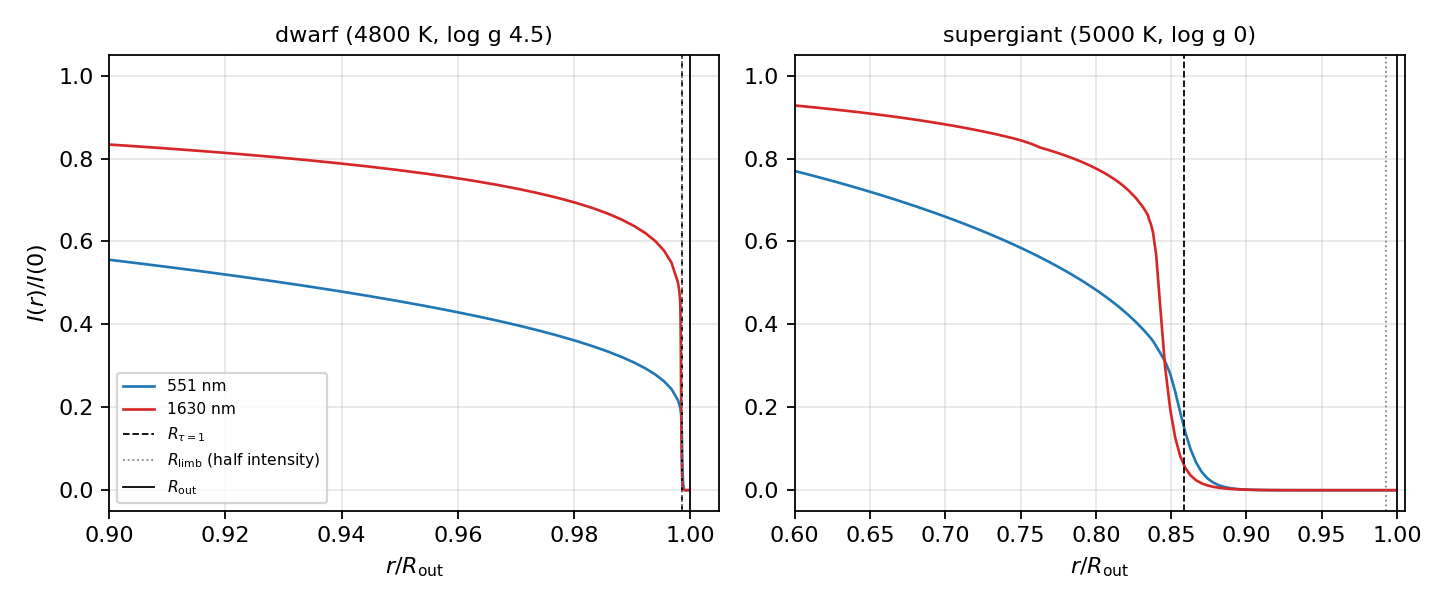
\includegraphics[width=\textwidth]{fig_limb.png}
\caption{Centre-to-limb intensity of the two stand-in NewEra models at
551 and 1630~nm against radius in units of the model's outer boundary,
with the Rosseland $\tau = 1$ radius (dashed), the apparent limb where
the continuum intensity halves (dotted) and the outer boundary
(solid). For the dwarf the three coincide to 0.14\%; for the
supergiant the visible limb lies 13.5\% outside $\tau = 1$.}
\label{fig:limb}
\end{figure}

\begin{table}[h]
\centering
\caption{Limb geometry and uniform-disk ratios of the stand-in models
($x = 1.5$, 4~m pupils).}
\begin{tabular}{lcccc}
\toprule
model & $R_{\rm out}/R_{\tau=1}$ & $R_{\rm out}/R_{\rm limb}$ & $\theta_{\rm UD}/\theta_{\rm LD}$ ($V$) & ($H$) \\
\midrule
4800 K, $\log g = 4.5$ (dwarf) & 1.0014 & 1.0014 & 0.927 & 0.971 \\
5000 K, $\log g = 0$ (supergiant) & 1.165 & 1.0076 & 0.924 & 0.963 \\
\bottomrule
\end{tabular}
\end{table}

The paper's $s$ multiplies a SATLAS profile normalized to a reference
diameter, and its $\sigma_s$ is compared directly with PIONIER's
limb-darkened diameters. Which radius the reference is matters at the
per-cent level for a giant (Fig.~\ref{fig:limb}): the profile shape
moves $\theta_{\rm UD}/\theta_{\rm LD}$ by only 0.3\% ($V$) to 0.8\%
($H$) between the two extreme gravities, but the definition of ``the
radius'' moves by 16\%. An II validation at 1\% must fit the same
profile with the same radius definition as the PIONIER analysis, or
it compares conventions rather than stars.

\subsection{Multiplexing}

\begin{figure}[h]
\centering
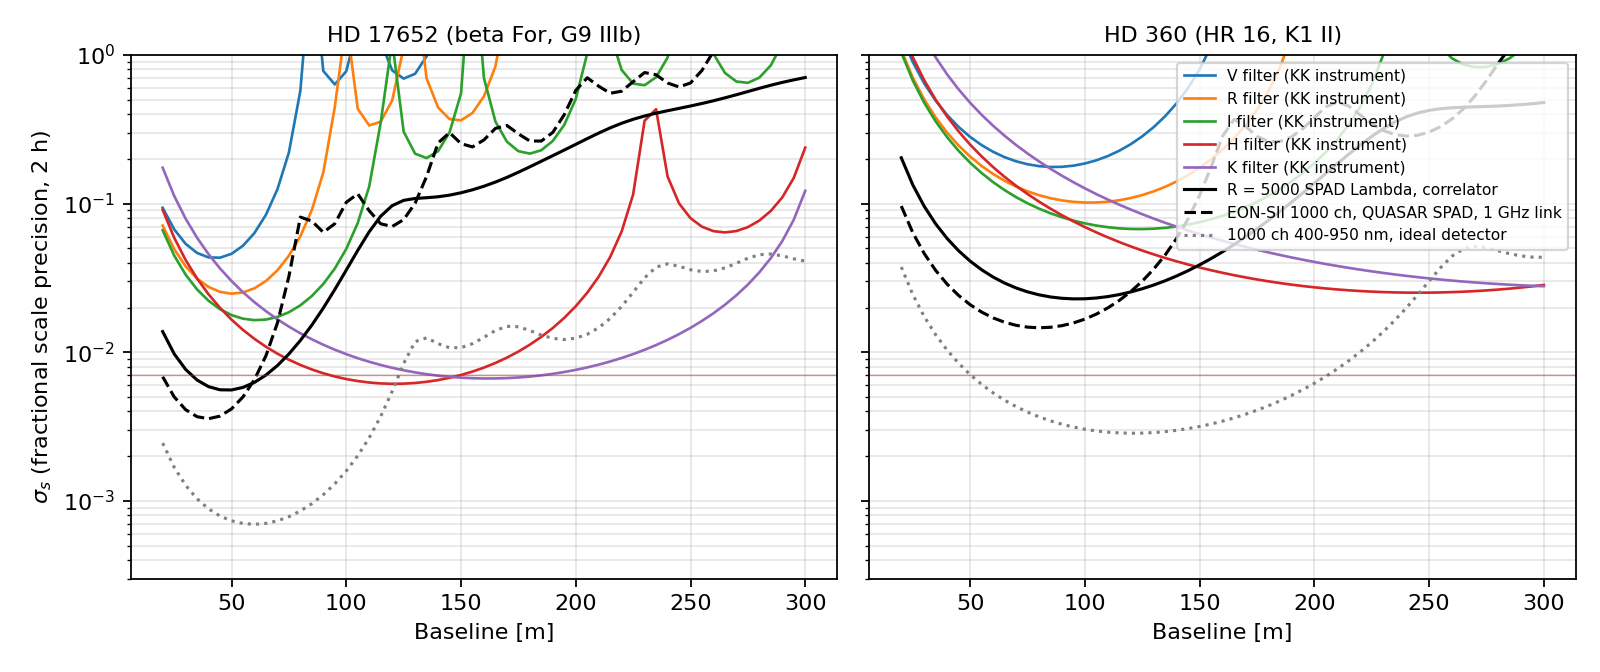
\includegraphics[width=\textwidth]{fig_sigma_s.png}
\caption{$\sigma_s$ against baseline in 2~h: the paper's single
filters (colours) and three multiplexed optical backends (black and
grey), dwarf stand-in profile. The thin red line is the paper's
$\sigma_s = 0.007$. Beyond $\sim$60~m (HD~17652) the optical channels
pass through the first null, hence the structure. The grey dotted
curve is their ideal detector (unit PDE, 42~ps) with 1000 channels:
that is the ``factor $\sim$100'' in time. Real detectors give parity
(the $R = 5000$ SPAD~Lambda correlator) to $\times3$ in time (EON-SII).}
\label{fig:sigma}
\end{figure}

\begin{table}[h]
\centering
\caption{Best $\sigma_s$ in 2~h and hours to $\sigma_s = 0.007$ (scaling
as $1/T$).}
\footnotesize
\begin{tabular}{lcc}
\toprule
backend & HD 17652 & HD 360 \\
\midrule
KK instrument, one H filter & 0.0061 (120 m) $\to$ 1.5 h & 0.025 (245 m) $\to$ 26 h \\
ideal detector, 1000 ch 400--950 nm & 0.0007 (60 m) $\to$ 0.02 h & 0.0029 (120 m) $\to$ 0.33 h \\
SPAD Lambda 320 ch, time-tag & 0.10 $\to$ 430 h & 0.10 $\to$ 430 h \\
SPAD Lambda 320 ch, correlator & 0.021 $\to$ 18 h & 0.084 $\to$ 290 h \\
$R = 5000$ (4325 ch), correlator & 0.0056 (50 m) $\to$ 1.3 h & 0.023 (95 m) $\to$ 21 h \\
$R = 5000$, correlator + PBS & 0.0040 $\to$ 0.64 h & 0.016 $\to$ 11 h \\
EON-SII 1000 ch, QUASAR SPAD, 1 GHz link & \textbf{0.0036 (40 m) $\to$ 0.52 h} & \textbf{0.015 (80 m) $\to$ 8.7 h} \\
\bottomrule
\end{tabular}
\end{table}

Two practical points: the optical channels do their work at 40--120~m,
inside the PIONIER-like baselines, whereas HD~360 needs 245~m in $H$;
and the H-band case itself requires an infrared photon counter with
picosecond jitter (InGaAs SPAD, SNSPD) that has not been modelled.

\subsection{Chromaticity}

\begin{figure}[h]
\centering
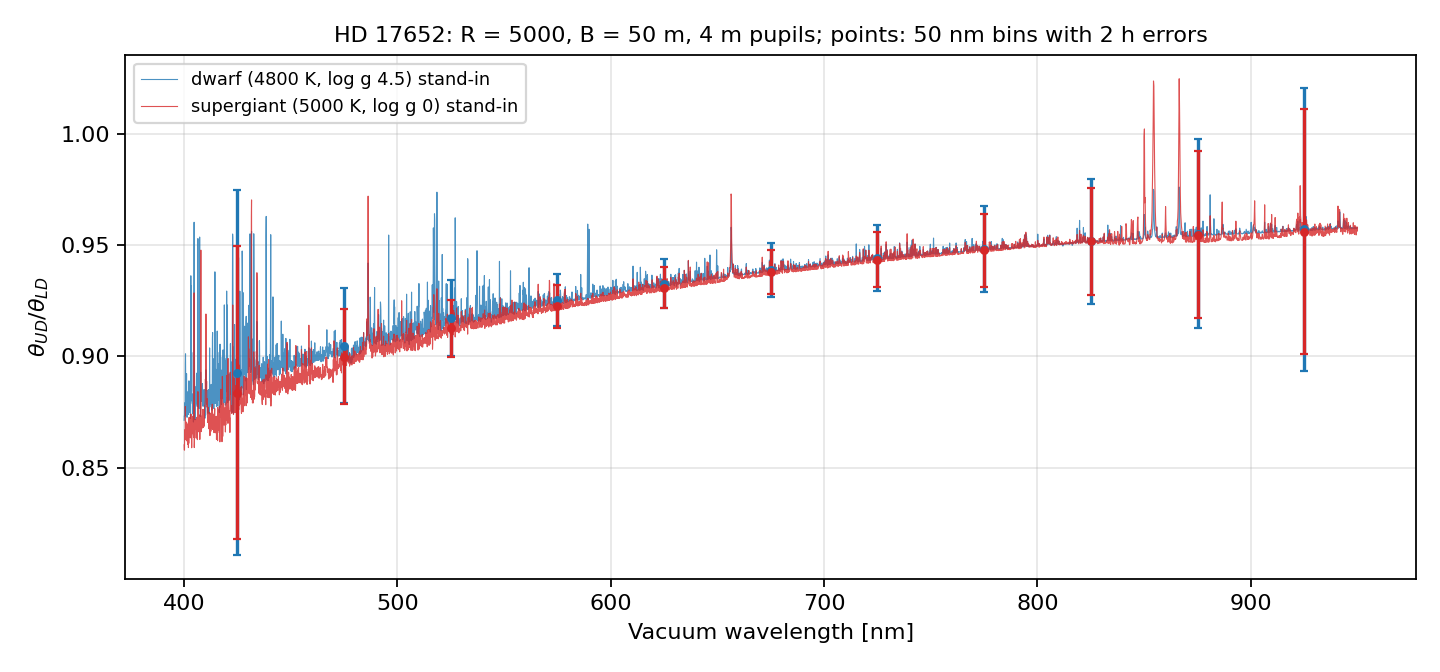
\includegraphics[width=\textwidth]{fig_chromatic.png}
\caption{$\theta_{\rm UD}/\theta_{\rm LD}$ per $R = 5000$ channel for
HD~17652 at $B = 50$~m with 4~m pupils, for both stand-in profiles;
points are inverse-variance means in 50~nm bins with the 2~h errors
of the $R = 5000$ correlator backend. The errors grow to the red
because 50~m barely resolves the star there (the optimum baseline is
band-dependent); the strong lines (Ca~II H and K, the G band, Mg~b,
H$\alpha$, the Ca~II triplet) stand 2--4\% above the continuum.}
\label{fig:chrom}
\end{figure}

The uniform-disk diameter runs 6\% across 400--950~nm (0.891, 0.903,
0.917, 0.929, 0.944, 0.955 in the bins 400--450, 450--500, 500--550,
550--650, 650--800, 800--950~nm). The two stand-ins differ by $\le
1$\% in the continuum. With $\sigma(\theta_{\rm UD})/\theta = 0.45$
per channel in 2~h on HD~17652, 50~nm bins reach $\sim$2\% and the
continuum slope is a $\sim$3$\sigma$ measurement per 2~h ($\sim$7$\sigma$
per night): the limb darkening of a K giant measured rather than
assumed, which is the test the authors say G/K atmospheres need.

\section{To do}
\label{sec:todo}

\begin{itemize}
\item \todo{Request the red-clump models from Hamburg} (P.~Hauschildt,
  E.~Baron; Hauschildt is away until 10~October 2026): NewEra HSR-RF at
  $[{\rm M/H}] = 0$ for $T_{\rm eff} = 4700, 4800, 4900$~K $\times$
  $\log g = 2.0, 2.5, 3.0$ (nine models), optionally 4800~K /
  $\log g = 2.5$ at $[{\rm M/H}] = -0.5$ and $+0.5$. Then: bin at NERSC
  (\texttt{tools/bin\_redclump.sh}, both wavelength ranges), rerun
  \texttt{scripts/redclump\_ii.py} and \texttt{redclump\_figures.py},
  and replace every stand-in number here. The gravity dependence of
  $R_{\rm limb}/R_{\tau=1}$ is the number this note cannot give.
\item \todo{Match the PIONIER convention.} Establish which radius the
  Gallenne et al.\ SATLAS fits report (the SATLAS reference radius vs
  the visible limb) and evaluate the NewEra giant's profile with the
  same definition before quoting a diameter offset.
\item \todo{Photometry check.} With $\theta_{\rm LD}$ and the stand-in
  fluxes the model $V$ is 0.18~mag brighter than observed (0.34 with
  the supergiant's larger drawn disk); see whether the giant model and
  metallicity close this.
\item \todo{H-band detector.} Add an InGaAs-SPAD / SNSPD preset (PDE
  curve, jitter, dark rate, dead time) so that the H-band case is
  computed with the same realism as the optical ones.
\item \todo{Observation realism.} Baseline projection over the 2~h,
  atmospheric extinction and airmass, and a Monte Carlo of the $s$ fit
  (\texttt{hbtsim.montecarlo}) with the singles-based normalization, to
  check that the Cram\'er--Rao bound is attained.
\item \todo{CTAO case.} Their ``666 baselines'' with the actual SST
  layout (\texttt{bispectrum.Array}): redundancy, projected baselines
  over the night, second-lobe coverage across channels.
\end{itemize}

\paragraph{Code and logs.} In the repository \texttt{nugent68/binary}
(commit \texttt{e8a197f} and following):
\begin{itemize}\setlength{\itemsep}{0pt}
\item \texttt{hbtsim/diameter.py}; \texttt{hbtsim/single.py} (\texttt{HD\_17652}, \texttt{HD\_360})
\item \texttt{scripts/redclump\_ii.py}, \texttt{scripts/redclump\_figures.py}
\item \texttt{output/logs/redclump\_ii\_dwarf.txt}, \texttt{redclump\_ii\_supergiant.txt}
\item \texttt{docs/redclump\_ii.md} (the same results in Markdown)
\end{itemize}

\end{document}
